% !TEX root = ./setup.tex

\section{System Description} \label{System_Description}
Identification Rumble's technical architecture, on a high level, is comprised of the following hardware and software components:

\begin{itemize}
  \item Tangible hardware (identity card replicas)
  \item Static hardware (RFID readers, screens and their connected computer)
  \item Station software (language, dilemma and evaluation station)
  \item Central backend API
\end{itemize}

Software components are realized using web technologies.
JavaScript\footnote{\url{https://developer.mozilla.org/bm/docs/Web/JavaScript}, Accessed: 07-02-2018} is used for front-facing parts of the prototype i.e. stations museum visitors interact with.
This implies that computers used in these stations are capable to run a browser (See Figure \ref{fig:architecture}).
As this project is not a traditionally published website, for visitors using a variety of browsers, no special support has been implemented for edge cases and old browsers.
Instead, the museum is in full control which browsers are deployed.
Currently, recent versions (i.e. last 2) of the following browsers are guaranteed to be supported\footnote{Other browsers and versions can be able to run the prototype as well}:

\begin{itemize}
  \item Google Chrome\footnote{\url{https://www.google.ca/intl/en/chrome/}, Accessed: 07-02-2018}
  \item Mozilla Firefox\footnote{\url{https://www.mozilla.org/en-US/firefox/new}, Accessed: 07-02-2018}
  \item Microsoft Edge\footnote{\url{https://www.microsoft.com/en-us/windows/microsoft-edge}, Accessed: 07-02-2018}
\end{itemize}

Given these constraints, the stakeholder is able to choose any device capable of running these browsers.

The central backend uses Node.js\footnote{\url{https://nodejs.org, Accessed: 07-02-2018}} as its framework and runs TypeScript\footnote{\url{https://www.typescriptlang.org}, Accessed: 07-02-2018} which is a strongly typed superset of JavaScript.
More on this component in section \ref{sec:backend}.

Figure \ref{fig:architecture} visualizes the full system and distinguishes between physical and digital components.
The following sections elaborate on the different parts found in the diagram.
Furthermore, every number corresponds to one of the following sections in ascending order.
This will be made explicit in each section as well.


\subsection{Identity Card Replica} \label{sec:idcardreplica}
Every physical identity card is equipped with an RFID tag inside (Figure \ref{fig:architecture}, marker 1).
These replicas are modeled after the \textit{'persoonsbewijs'} which Dutch citizens were required to carry with them during the German occupation in WWII\footnote{\url{http://www.persoonsbewijzen.nl/} (Dutch), Accessed: 09-02-2018}.
An interactive, visual representation of these identity cards can be found here:

\begin{flushleft}
  \url{https://identification-rumble.science/persoonsbewijs}\footnote{Accessed: 07-02-2018}
\end{flushleft}

Due to the contained RFID tags, these identity cards can be recognized by RFID readers.
Within the range of communication, up to 6cm\footnote{\url{https://www.phidgets.com/?tier=3&catid=81&pcid=72&prodid=23}, Accessed: 07-02-2018}, the scanners are able to read the digital value stored on tags.
With the exception of two tags, the ones used in this prototype are read-only.
Therefore, a simple mapping between the predefined values on the tags to their digital representation can be performed.
Digital identity cards have a unique integer number assigned to them from which they can be retrieved.

\begin{lstlisting}[caption={JavaScript mapping for RFID tags}, label={lst:mapping}, language=JavaScript]
{
  '79001ff8c8': {
    name: 'Card',
    value: 0
  },
  '4a0037db70': {
    name: 'Blue chip',
    value: 1
  },
  ...
}
\end{lstlisting}

In listing \ref{lst:mapping}, a simple JavaScript object uses the RFID tags as its keys.
Each key maps to a descriptive name and a value which represents a unique number of a digital identity card.
The name is merely for administration purposes and helps to identify the physical tag in the mapping interface (See Figure \ref{fig:mappinginterface}).

\begin{figure}[h]
  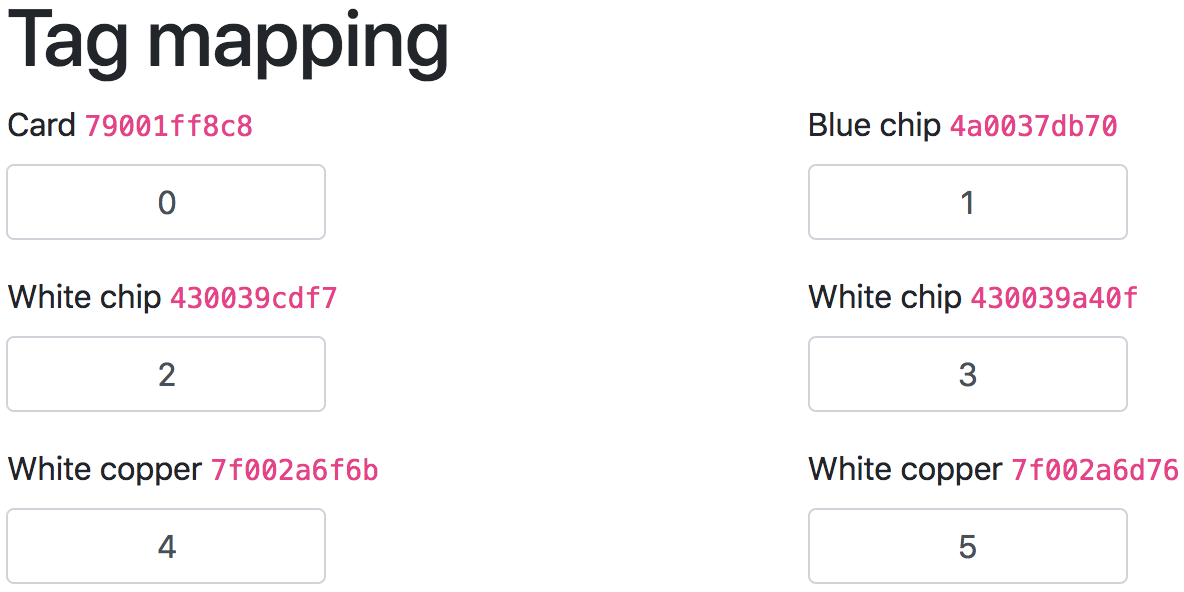
\includegraphics[width=5cm]{assets/mapping-interface.png}
  \caption{Tag mapping interface}
  \centering
  \label{fig:mappinginterface}
\end{figure}


\subsection{Language Scanner}
This station allows visitors to change the language of their experience according to their preference.
Every supported language of the museum is represented by a small physical flag (roughly the size of an identity card).
Each of these flags is equipped with an RFID reader (Figure \ref{fig:architecture}, marker 2).
Upon holding an identity card close to a flag the corresponding tag is recognized.
As previously discussed (Section \ref{sec:idcardreplica}) this tag is then mapped to its corresponding digital identity card.
Finally, the station signals the backend to change the language of this identity card accordingly.
In addition to that, it emits an audible beep noise indicating successful execution.

Changing languages in the prototype is possible at:

\begin{flushleft}
  \url{https://identification-rumble.science/language}\footnote{Accessed: 07-02-2018}
\end{flushleft}


\subsection{Dilemma Station}
Dilemmas require the most hardware in the Identification Rumble prototype.
They consist of a screen, computer and RFID reader for every possible answer.
While the current design only uses two answers, it is possible to provide more choices.
This setup is repeated for every dilemma in the exhibition (Figure \ref{fig:architecture}, marker 3).

In its idle state, the station prompts visitors to hold their identity cards to either of the connected RFID readers.
Scanning the identity card allows the system to retrieve the previously selected language of the visitor.
It continues by playing the corresponding dilemma animation video in the correct language.

Dilemma videos are virtually segmented into three parts:
(1) story, (2) answer prompt and (3) outro.
During the first story segment, the station ignores any recognized identity cards on the RFID readers.
Once it reaches the answer prompt section, scanning an identity card will fast forward the video to the outro.
Finally, the outro provides contextual information to the visitor and concludes the story.
Scanning a different identity card during the outro or after the animation has finished restarts this process.

Answering a dilemma leads to the station sending relevant information to the backend; namely respective IDs of the dilemma, answer and identity card.

This part of the prototype can be found at:

\begin{flushleft}
  \url{https://identification-rumble.science/dilemmas}\footnote{Accessed: 07-02-2018}
\end{flushleft}


\subsection{Evaluation Station} \label{sec:evaluationstation}
The Evaluation Station consists of a screen, RFID reader and computer each (Figure \ref{fig:architecture}, marker 4).
Technically speaking only one station is required to provide the functionality to visitors.
However, depending on the number of visitors trying to access this station at the same time the setup can be repeated.

Scanning an identity card at this station sets it off to fetch two data objects from the backend: (1) selected answers of this identity card and (2) historical statistics of other visitors selected languages and answers.
This information is used to compare personal choices with previous visitors who answered the same.

\begin{lstlisting}[caption={Calculating percentage of visitors who answered the same}, label={lst:samepercentage}, language=JavaScript]
// this.stats.dilemmas: Object<Number, Array<Date>>
const answerStats = this.stats.dilemmas[dilemmaId];
const totalAnswers = Object.values(answerStats).reduce(
    (sum, dates) => sum + dates.length,
    0
);
const sameAnswersCount = answerStats[answerId].length;
const percent = Math.round(
    sameAnswersCount / totalAnswers * 100
);
\end{lstlisting}

In listing \ref{lst:samepercentage}, the percentage comparison is calculated by accessing the answer statistics of an individual dilemma.
Each answer can be inspected by using its ID and contains an array of dates indicating when it was selected.
Counting the total number of dates as well as the number of visitors answering the same allows calculating the final percentage.

Apart from that, two types of charts are shown to visualize answer distribution (vertical bar chart) and the ratio of languages (pie chart).
These charts are realized using the Chartist\footnote{\url{https://gionkunz.github.io/chartist-js/}, Accessed: 08-02-2018} library.

Evaluating choices of an identity card is possible at:

\begin{flushleft}
  \url{https://identification-rumble.science/evaluation}
\end{flushleft}


\subsection{Communication} \label{sec:communication}
Different parts of the system are scattered throughout the exhibition.
In order to trigger actions (language scanner, dilemma station) or fetch information (evaluation station) they have to contact the central backend server.
Therefore, each page starts a bi-directional WebSocket\footnote{\url{https://developer.mozilla.org/en-US/docs/Web/API/WebSocket}, Accessed: 08-02-2018} connection with the server.
As connection loss is not handled by the native WebSocket browser API and to ease usage Socket.IO\footnote{\url{https://socket.io/}, Accessed: 08-02-2018} is used as a library (Figure \ref{fig:architecture}, marker 5).
It provides an event based interface to send data from the client to the server or vice versa.


\subsection{Backend} \label{sec:backend}
The backend API is implemented in TypeScript using Node.js as a framework and runtime (Figure \ref{fig:architecture}, marker 6).
It acts as the central communication unit to which all parts of the system report their changes and can retrieve data.
Responsibility of the backend can be divided into three distinct categories: (1) providing the Socket.IO server (Section \ref{sec:communication}), (2) implementing business logic and (3) persisting state (Section \ref{sec:storage}).

As soon as a client opens a new connection with the Socket.IO server it begins to listen for all possible events.
These events are delegated to their corresponding business logic services.
Table \ref{tbl:eventservices} provides a full overview of event and parameter delegation to services.
While it refers to identity cards the backend code uses the legacy term 'passport' which was used during the conception of the project.

\begin{table}
  \centering
  \begin{tabular}{ |l|l| }
    \hline
    \textbf{Event + Parameters} & \textbf{Service} \\
    \hline
    getPassports() & passport \\
    createPassport() & passport \\
    resetPassport(id) & passport \\
    removePassport(id) & passport \\
    getPassport(id) & passport \\
    changeLanguage(passportId, languageCode) & passport \\
    answerDilemma(passportId, dilemmaId, answerId) & passport \\
    getStats() & statistics \\
    setReadOnlyMode(password, enabled) & settings \\
    getReadOnlyMode() & settings \\
    getTagMapping() & settings \\
    setTagMapping(tag, value) & settings \\
    \hline
  \end{tabular}
  \caption{Delegation of events and parameters to services} \label{tbl:eventservices}
\end{table}


\begin{figure*}
  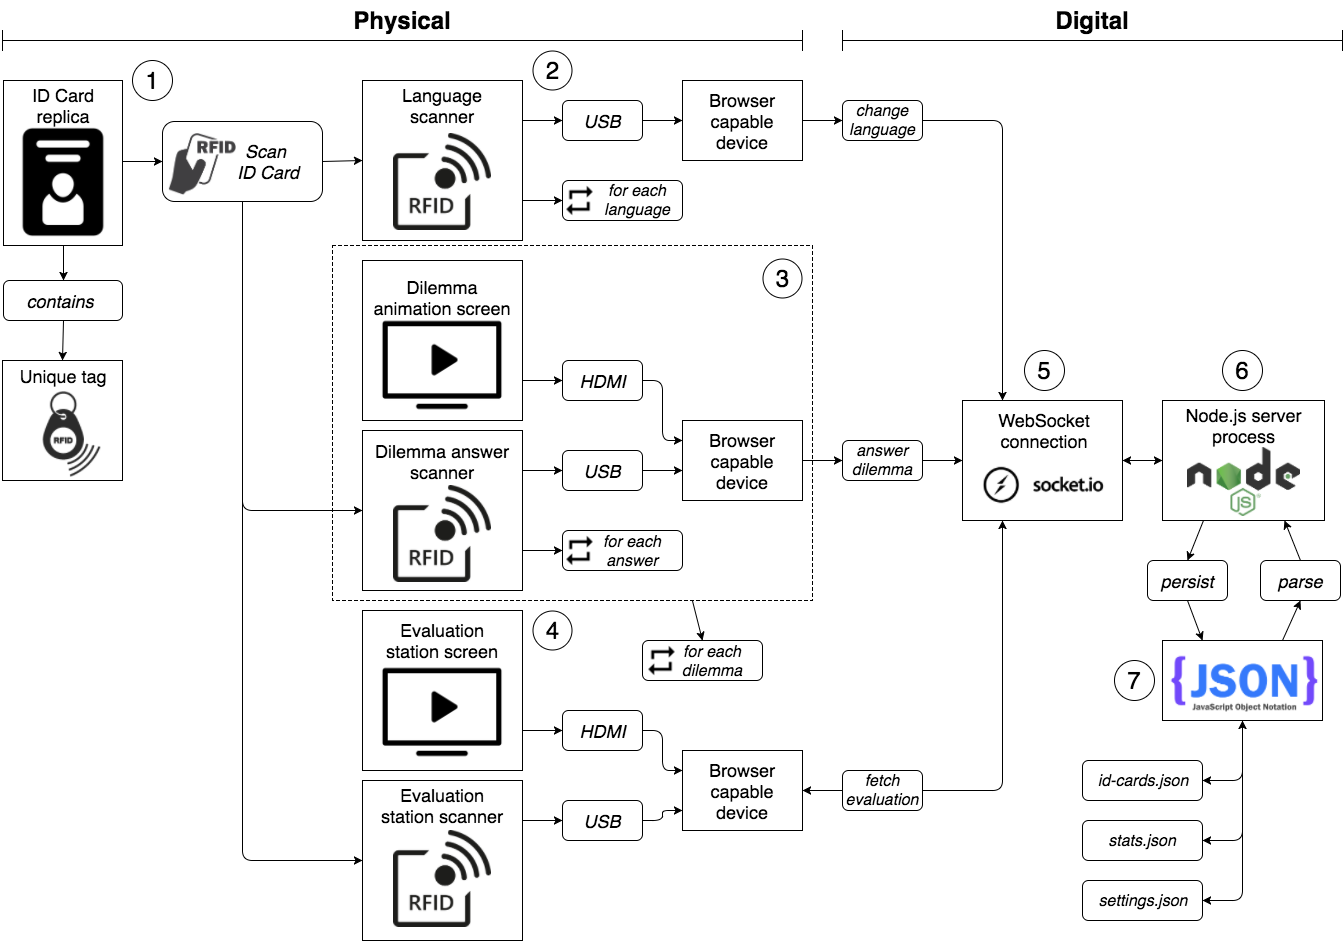
\includegraphics[width=15cm,keepaspectratio]{assets/system-architecture.png}
  \caption{System architecture}
  \label{fig:architecture}
\end{figure*}

The passport service implements a straightforward CRUD\footnote{\url{https://developer.mozilla.org/en-US/docs/Glossary/CRUD}, Accessed: 09-02-2018} (Create, Read, Update, Delete) interface for accessing and manipulating identity cards.
Changing language and answering a dilemma are the two main mutation functions operating on the state of an identity card.
They notify the statistics service of their changes in the background which in turn allow them to provide historical data for the evaluation station (Section \ref{sec:evaluationstation}).

Administrative functionality is handled within the settings service.
It contains a boolean flag indicating whether the system is in a read-only mode disabling creation and deletion of identity cards as well as changes to the tag mapping.
This can be used for presentation purposes or to prevent accidental changes.
Furthermore, the tag mapping discussed in section \ref{sec:idcardreplica} is handled by the settings service.

Restarting the backend should not lead to unexpected data loss.
Therefore, services continuously persist their own state after changes have been made (Section \ref{sec:storage}).


\subsection{Storage} \label{sec:storage}
Persisting state is implemented using plain JSON\footnote{\url{https://www.json.org/}, Accessed: 09-02-2018} (JavaScript Object Notation) files for each service (Figure \ref{fig:architecture}, marker 7).
Before the backend starts to accept connections the services try to parse previous state from these files.
When changes are committed to identity cards, statistics or system settings the respective service triggers an asynchronous write operation of its state.
Executing this operation asynchronously allows the backend to deal with different tasks in the mean time; this is a strong suit of Node.js.

It could be argued that relying on JSON serialization and parsing does not scale well and is inferior to a full blown database system.
While this is true for larger software systems this prototype intentionally avoids database system in spirit of the KISS-principle\footnote{\url{https://people.apache.org/~fhanik/kiss.html}, Accessed: 09-02-2018} (Keep It Simple, Stupid).
KISS is usually applied to code itself but can be adapted to other areas as well, in this case the setup of a software system.
Using a full database system increases the complexity of setup and maintaining the backup.
In addition to that, there is virtually no added value as this system only handles a limited amount of data.
Even with a generous estimate of 100 created identity cards storing their state would still be possible within the constraints of JSON files.
Special query functionality provided by database systems would still not be required as the backend performs lookups in memory.



